% !TeX encoding = UTF-8
% !TeX spellcheck = pl_PL

% $Id:$

%Author: Wojciech Domski
%Szablon do ząłożeń projektowych, raportu i dokumentacji z steorwników robotów
%Wersja v.1.0.0
%


%% Konfiguracja:
\newcommand{\kurs}{Sterowniki robot\'{o}w}
\newcommand{\formakursu}{Projekt}

%odkomentuj właściwy typ projektu
%\newcommand{\doctype}{Za\l{}o\.{z}enia projektowe}
\newcommand{\doctype}{Raport}
%\newcommand{\doctype}{Dokumentacja}

%wpisz nazwę projektu
\newcommand{\projectname}{Modu\l  Antykradzie\.{z}owy SMS}

%wpisz akronim projektu
\newcommand{\acronim}{MASS}

%zmaiast X wpisz numer grupy projektowej
\newcommand{\nrgrupy}{5}
%wpisz Imię i nazwisko oraz numer albumu
\newcommand{\osobaA}{Krzysztof \textsc{D\k{a}bek}, 218549}
%w przypadku projektu jednoosobowego usuń zawartość nowej komendy
\newcommand{\osobaB}{Maciej \textsc{Flis}, 218543}

%wpisz termin w formie, jak poniżej dzień, parzystość, godzina
\newcommand{\termin}{srTP11}

%wpisz imię i nazwisko prowadzącego
\newcommand{\prowadzacy}{mgr in\.{z}. Wojciech \textsc{Domski}}

\documentclass[10pt, a4paper]{article}
% W nawiasie klamrowym podana jest klasa dokumentu. Standardowe klasy artykułu
% to: article, amsart, scrartcl, artikel1, artikel2, artikel3.
% W nawiasie prostokątnym deklarowane są opcje dokumentu. Zamiast 10pt
% można podać 11pt lub 12pt. Dokument w dwóch kolumnach uzyskuje się po
% wpisaniu opcji twocolumn, 

%Preambuła dokumentu
\usepackage[final]{pdfpages}
% linki w spisie tresci, bibliografi
\usepackage[bookmarks=true,bookmarksnumbered=false,unicode=true,pdftex=true, colorlinks,filecolor=black,linkcolor=black,urlcolor=black,citecolor=black]{hyperref}

%ustawienie rozmiaru papieru
\usepackage[a4paper, left=2.5cm, right=2.5cm, top=2.5cm, bottom=2.5cm, headsep=1.2cm]{geometry}

%rozmaite ustawienia pozwalające okreslić język

%NALEŻY wybrać jeden z pakietów
%\usepackage{polski} %przydatne podczas składania dokumentów w j. polskim
\usepackage[polish]{babel}  % pakiet lokalizujący dokument w języku polskim
%\usepackage[british]{babel}

\usepackage{indentfirst}	% polski styl pisania (np. rozpoczecie pierwszego akapitu
% pod nazwa rozdzialu od wciecia)
%\usepackage[OT4]{fontenc}
\usepackage[utf8]{inputenc} % w miejsce utf8 można wpisać latin2 bądź cp1250,
% w zależności od tego w jaki sposób kodowane są 
% polskie znaki diakrytyczne przy wprowadzaniu 
% z klawiatury.
%kodowanie znaków, zależne od systemu
\usepackage[T1]{fontenc} %poprawne składanie polskich czcionek

%OPEROWANIE NA OBRAZACH
\usepackage{graphicx}       % pakiet graficzny, umożliwiający m.in.
% import grafik w formacie eps
%\usepackage{epstopdf}		% pozwala na importowanie grafik w formacie eps
% przy użyciu pdflatex
\usepackage[update,prepend]{epstopdf}
\usepackage{rotating}       % pakiet umożliwiający obracanie rysunków
\usepackage{subfigure}      % pakiet umożliwiający tworzenie podrysunków
\usepackage{epic}           % pakiet umożliwiający rysowanie w środowisku latex
\usepackage{psfrag}         % pakiet umożliwiający podmianę łańcuchów znaków 
% w plikach eps
%\usepackage{curves}         % pakiet do wykreslania krzywych

%pakiety dodające dużo dodatkowych poleceń matematycznych
\usepackage{amsfonts}       % pakiet z rozmaitymi czcionkami matematycznymi
%\usepackage{amssymb}        % pakiet z rozmaitymi symbolami matematycznymi
\usepackage{amsmath}        % pakiet z rozmaitymi środowiskami matematycznymi

\usepackage{fp}             % pakiet z funkcjami operujacymi 
% na liczbach zmiennoprzecinkowych
\usepackage{calc}           % pakiet umożliwiający operacje arytmetyczne
% na tzw. licznikach (liczbach całkowitych)
\usepackage{leftidx}		% indeksy górne i dolne po lewej stronie

%definicje matematyczne
\providecommand{\abs}[1]{\lvert#1\rvert}
\providecommand{\norm}[1]{\lVert#1\rVert}

%pakiety wspomagające i poprawiające składanie tabel
\usepackage{supertabular}
\usepackage{array}
\usepackage{tabularx}
\usepackage{hhline}
\usepackage{longtable}		% wsparcie dla dlugich tabel
\usepackage{multicol}		% podzial strony na wiele kolumn

%pakiet do BibTex
\usepackage{cite}

\usepackage{url} %pakiet pozawalający na dodawanie adresów url w bibliografi

%pakiet wypisujący na marginesie etykiety równań i rysunków zdefiniowanych przez \label{}, chcąc wygenerować finalną wersję dokumentu wystarczy usunąć poniższą linię
%\usepackage{showlabels}

\usepackage{float}			% lepsza obsluga mechanizmow obiektow plywajacych
% wymuszenie wstawienia np. tabeli, obrazka w danym miejscu przez [H]

\usepackage{listings}       % pakiet dedykowany zrodlom programow
\usepackage{color}


\definecolor{dkgreen}{rgb}{0,0.6,0}
\definecolor{gray}{rgb}{0.5,0.5,0.5}
\definecolor{mauve}{rgb}{0.58,0,0.82}

\lstset{ %
	language=Matlab,                % the language of the code
	basicstyle=\scriptsize,           % the size of the fonts that are used for the code
	numbers=left,                   % where to put the line-numbers
	numberstyle=\tiny\color{gray},  % the style that is used for the line-numbers
	stepnumber=1,                   % the step between two line-numbers. If it's 1, each line 
	% will be numbered
	numbersep=5pt,                  % how far the line-numbers are from the code
	backgroundcolor=\color{white},      % choose the background color. You must add \usepackage{color}
	showspaces=false,               % show spaces adding particular underscores
	showstringspaces=false,         % underline spaces within strings
	showtabs=false,                 % show tabs within strings adding particular underscores
	%frame=single,                   % adds a frame around the code
	rulecolor=\color{black},        % if not set, the frame-color may be changed on line-breaks within not-black text (e.g. comments (green here))
	tabsize=2,                      % sets default tabsize to 2 spaces
	captionpos=b,                   % sets the caption-position to bottom
	breaklines=true,                % sets automatic line breaking
	breakatwhitespace=false,        % sets if automatic breaks should only happen at whitespace
	%title=\lstname,                   % show the filename of files included with \lstinputlisting;
	% also try caption instead of title
	keywordstyle=\color{blue},          % keyword style
	commentstyle=\color{dkgreen},       % comment style
	stringstyle=\color{mauve},         % string literal style
	escapeinside={\%*}{*)},            % if you want to add LaTeX within your code
	morekeywords={*,...},              % if you want to add more keywords to the set
	deletekeywords={...}              % if you want to delete keywords from the given language
}

%polish signs in lst code
\lstset{literate=%
	{ą}{{\k{a}}}1
	{ć}{{\'c}}1
	{ę}{{\k{e}}}1
	{ł}{{\l}}1
	{ń}{{\'n}}1
	{ó}{{\'o}}1
	{ś}{{\'s}}1
	{ż}{{\.z}}1
	{ź}{{\'z}}1
	{Ą}{{\k{A}}}1
	{Ć}{{\'C}}1
	{Ę}{{\k{E}}}1
	{Ł}{{\L}}1
	{Ń}{{\'N}}1
	{Ó}{{\'O}}1
	{Ś}{{\'S}}1
	{Ż}{{\.Z}}1
	{Ź}{{\'Z}}1
}

\usepackage{verbatim}       % pakiet dedykowany rozmaitym wydrukom tekstowym
\usepackage{ifthen}         % pakiet umożliwiający tworzenie prostych programów
% (m.in. zawiera instrukcje powtórzeniowe 
% i warunkowe)
\usepackage{upquote}		%normal quotations marks ' and `

% deklaracje wymagane przez pakiet theorem automatycznie ladowany w przypadku
% klasy dokumentu article
%
\newtheorem{Dn}{Definicja}[section]     % deklaracja srodowiska definicja
\newtheorem{La}[Dn]{Lemat}                % deklaracja srodowiska lemat
\newtheorem{Tm}[Dn]{Twierdzenie}          % deklaracja srodowiska twierdzenie
\newtheorem{Rk}[Dn]{Spostrze{\.z}enie}  % deklaracja srodowiska spostrzezenie
\newtheorem{Am}[Dn]{Algorytm}           % deklaracja srodowiska algorytm
\newtheorem{As}[Dn]{Za{\l}o{\.z}enie}   % deklaracja srodowiska zalozenie
\newtheorem{Pn}[Dn]{Propozycja}           % deklaracja srodowiska propozycja
\newtheorem{Py}[Dn]{W{\l}asno{\'s}{\'c}}  % deklaracja srodowiska wlasnosc
\newtheorem{Cy}[Dn]{Wniosek}              % deklaracja srodowiska wniosek
\newtheorem{Ee}[Dn]{Przyk{\l}ad}        % deklaracja srodowiska przyklad
\newtheorem{Ex}{{\'C}wiczenie}          % deklaracja srodowiska cwiczenie

%helps to specify width of a column in table
%\begin{tabular}{|C{1cm}|c|c|c|c|c|c|c|c|c|c|}
%first column will have widht of 1cm
\newcolumntype{L}[1]{>{\raggedright\let\newline\\\arraybackslash\hspace{0pt}}m{#1}}
\newcolumntype{C}[1]{>{\centering\let\newline\\\arraybackslash\hspace{0pt}}m{#1}}
\newcolumntype{R}[1]{>{\raggedleft\let\newline\\\arraybackslash\hspace{0pt}}m{#1}}

\sloppy			%zawija bardzo długie linie

\pagenumbering{gobble}% Remove page numbers (and reset to 1)
	
\begin{document}

\def\tablename{Tabela}	%zmienienie nazwy tabel z Tablica na Tabela

\begin{titlepage}
	\begin{center}
		\textsc{\LARGE \formakursu}\\[1cm]		
		\textsc{\Large \kurs}\\[0.5cm]		
		\rule{\textwidth}{0.08cm}\\[0.4cm]
		{\huge \bfseries \doctype}\\[1cm]
		{\huge \bfseries \projectname}\\[0.5cm]
		{\huge \bfseries \acronim}\\[0.4cm]
		\rule{\textwidth}{0.08cm}\\[1cm]
		
		\begin{flushright} \large
		\emph{Skład grupy (\nrgrupy):}\\
		\osobaA\\
		\osobaB\\[0.4cm]
		
		\emph{Termin: }\termin\\[0.4cm]

		\emph{Prowadzący:} \\
		\prowadzacy \\
		
		\end{flushright}
		
		\vfill
		
		{\large \today}
	\end{center}	
\end{titlepage}

\newpage
\tableofcontents
\newpage

\normalsize

\section{Główne założenia projektowe}
\begin{itemize}
\item Stworzenie software'owego projektu modułu antykradzieżowego na gotowej płytce, zaprojektowanej przez Macieja Flisa, opartej na mikrokontrolerze STM32F746VGT6.
\item Napisanie programu z użyciem biblioteki HAL generowanej przez dedykowane IDE od firmy ST (STM32 toolchain: STM32CubeMX, Atollic Truestudio).
\item Wgrywanie programu na płytkę za pomocą konwertera USB $\rightarrow$ UART.
\item Wykorzystanie modułu GPS do uzyskania lokalizacji płytki.
\item Wykorzystanie akcelerometru do uruchamiania wszystkich modułów w momencie poruszenia płytką.
\item Przesyłanie informacji na żądanie w wiadomości SMS z użyciem modułu GSM.
\item Emulacja pamięci EPROM w pamięci flash za pomocą bufora cyklicznego i zapisywanie w niej kolejnych lokalizacji modułu (po każdym przejściu w stan czuwania oraz co ustalony czas w stanie aktywnym).
\item Uruchomienie zegara czasu rzeczywistego (RTC) i zapisywanie informacji o czasie przeprowadzenia pomiaru wraz z lokalizacją w symulowanej pamięci EPROM w formie logu.
\item Wysyłanie danych z logu do komputera przez port USB.
\end{itemize}

\section{Harmonogram}
\begin{itemize}
\item (20.03. - 26.03.) Konfiguracja peryferiów mikrokontrolera, wygenerowanie kodu, wgranie programu na płytkę przez UART.
\item (27.03. - 2.04.) Oprogramowanie komunikacji USB i akcelerometru.
\item (3.04. - 23.04.) Uruchomienie modułu GSM, uruchomienie modułu GPS.
\item (24.04. - 7.05.) Oprogramowanie RTC, emulacja pamięci EPROM.
\item (8.05. - 14.05.) Juwenalia :)
\item (15.05. - 26.05) Przygotowanie raportu, przedstawienie pierwszego etapu prac nad projektem.
\item (27.05. - 11.06) Przygotowanie gotowej aplikacji, testy, rozwiązywanie problemów.
\item (12.06. - 22.06) Przygotowanie dokumentacji technicznej, przedstawienie gotowego projektu.
\end{itemize}

\section{Opis zrealizowanych prac}
Zadania zrealizowane na płytce stworzonej jako moduł antykradzieżowy opartej o mikrokontroler STM32F746VGT6:
\begin{itemize}
\item Konfiguracja mikrokontrolera i peryferiów.
\item Wgrywanie kodu na płytkę przez UART oraz SWD, debuggowanie.
\item Implementacja komunikacji przez USB.
\item Obsługa akcelerometru FXOS8700CQ.
\item Próby nawiązania połączenia z urządzeniem GSM Quectel M12 (na płytce).
\item Próby nawiązania połączenia z urządzeniem GPS Quectel L70 (na płytce).
\item Próby nawiązania połączenia z zewnętrznym modułem GSM.
\item Przesyłanie danych przez konwerter UART $\rightarrow$ USB.
\end{itemize}
Okazało się, że z powodu błędów projektowych związanych z hardwarem płytki, trzeba było dokonać zmiany koncepcji i używanych urządzeń. Zdecydowano się na:
\begin{itemize}
\item Płytkę rozwojową Kamami ZL41ARMF4 z mikrokontrolerem STM32F417VGT6.
\item Moduł z akcelerometrem MPU6050.
\item Moduł GSM, GPS Waveshare Sim808.
\end{itemize}
Zadania zrealizowane na modułach oraz płytce rozwojowej ZL41ARMF4:
\begin{itemize}
\item Pobieranie danych z GPS, komendy wysyłane z terminala komputera.
\item Wysyłanie SMS przez GSM, komendy wysyłane z terminala komputera.
\item Oprogramowanie akcelerometru MPU6050 (nietestowane).
\item Implementacja komunikacji przez USB.
\end{itemize}
Wykorzystany moduł Waveshare Sim808 prawdopodobnie został uszkodzony i przestał odpowiadać na komendy ''AT'', co uniemożliwiło dalsze prace związane z projektem oraz wykonanie wszystkich zadań zgodnie z harmonogramem.\\
W planach na najbliższe tygodnie jest zakupienie nowego modułu (modułów) GPS, GSM oraz nawiązanie z nim komunikacji i oprogramowanie tego na mikrokontrolerze. Następnie sprawdzenie i poprawienie obsługi akcelerometru, implementacja RTC oraz emulowanej pamięci EEPROM.

\section{Konfiguracja mikrokontrolera}
W projekcie wykorzystywana jest płytka rozwojowa ZL41ARMF4 z mikrokontrolerem STM32F417VGT6. Na płytce wyprowadzone są wszystkie piny mikrokontrolera, może być zasilana przez port miniUSB. Wygląd płytki został przedstawiony na rysunku \ref{fig:uC}.
\begin{figure}[!htb]
\centering
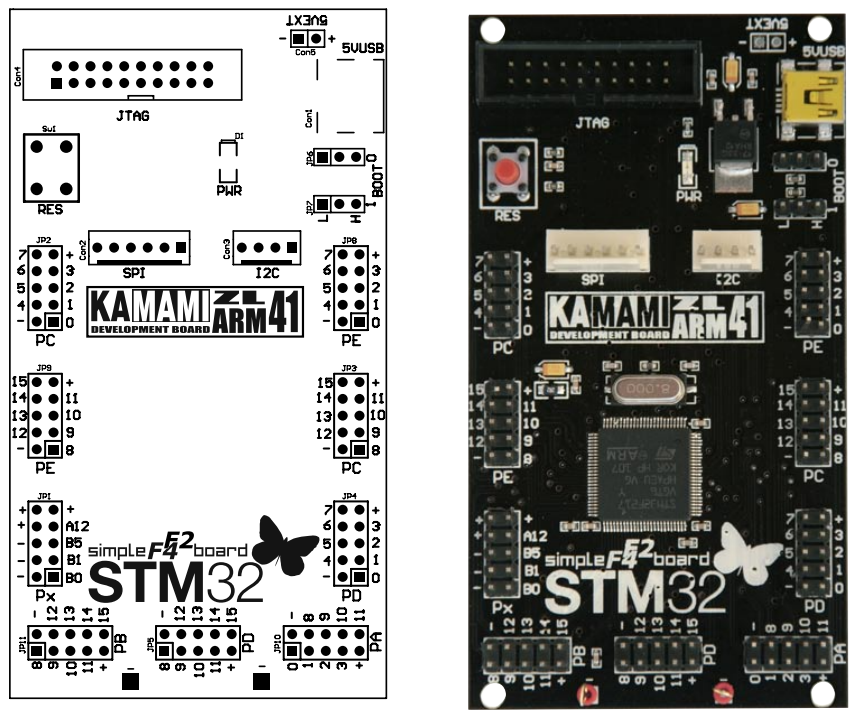
\includegraphics[height=0.43\textheight]{./uC.PNG}
\caption{Płytka rozwojowa Zl41ARMF4 od Kamami \label{fig:uC}}
\end{figure}\\
W konfiguracji pinów mikrokontrolera przewidziano:
\begin{itemize}
\item I2C (PB8 SCL, PB9 SDA) oraz wejście zewnętrznego przerwania (PE7) dla modułu z akcelerometrem.
\item UART (PC6 Tx, PC7 Rx) dla modułu SIM808 (GSM oraz GPS).
\item UART (PC10 Tx, PC11 Rx) dla komunikacji z komputerem przez zewnętrzny konwerter UART$\rightarrow$ USB.
\item USB (PA11 otg\textunderscore fs\textunderscore dm, PA12 otg\textunderscore fs\textunderscore dp) w trybie device do komunikacji przez Virtual COM Port.
\item RCC (PH0 osc\textunderscore in, PH1 osc\textunderscore out) zewnętrzny oscylator 8MHz dla US.
\item SWD (PA13 swdio, PA14 swclk) szeregowy port do debuggowania.
\end{itemize}

Konfiguracja pinów mikrokontrolera została przedstawiona na rysunku \ref{fig:uCconfig} oraz w tabeli \ref{tab:uCconfig}.\\
\begin{figure}[!htb]
\centering
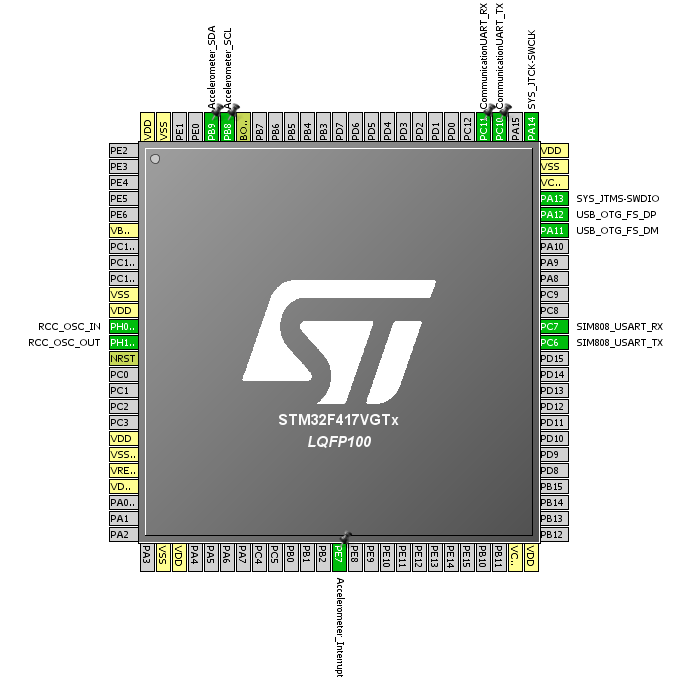
\includegraphics[height=0.6\textheight]{./KonfiguracjauC.PNG}
\caption{Konfiguracja mikrokontrolera (pinout) \label{fig:uCconfig}}
\end{figure}
\\
\begin{table}
\caption{Konfiguracja pinów mikrokontrolera \label{tab:uCconfig}}
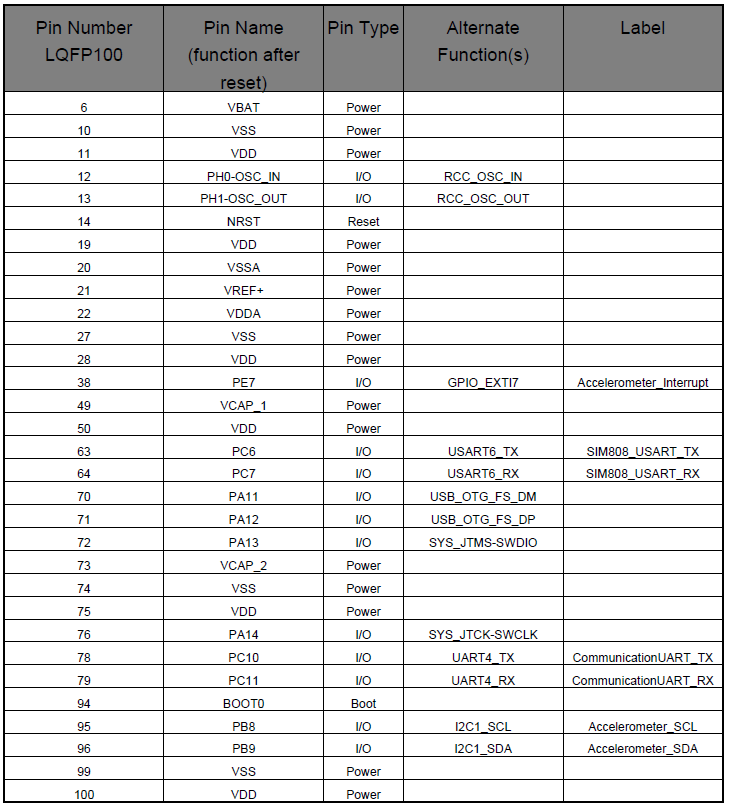
\includegraphics[width=\textwidth]{./KonfiguracjaPeryTab.PNG}
\end{table}
Konfiguracja zegara mikrokontrolera zakłada maksymalne możliwe taktowanie timerów oraz taktowanie 48MHz z wykorzystaniem HSE (oscylatora 8MHz) do obsługi USB.\\
Konfiguracja zegara mikrokontrolera została przedstawiona na rysunku \ref{fig:uCclock}
\begin{figure}[!htb]
\centering
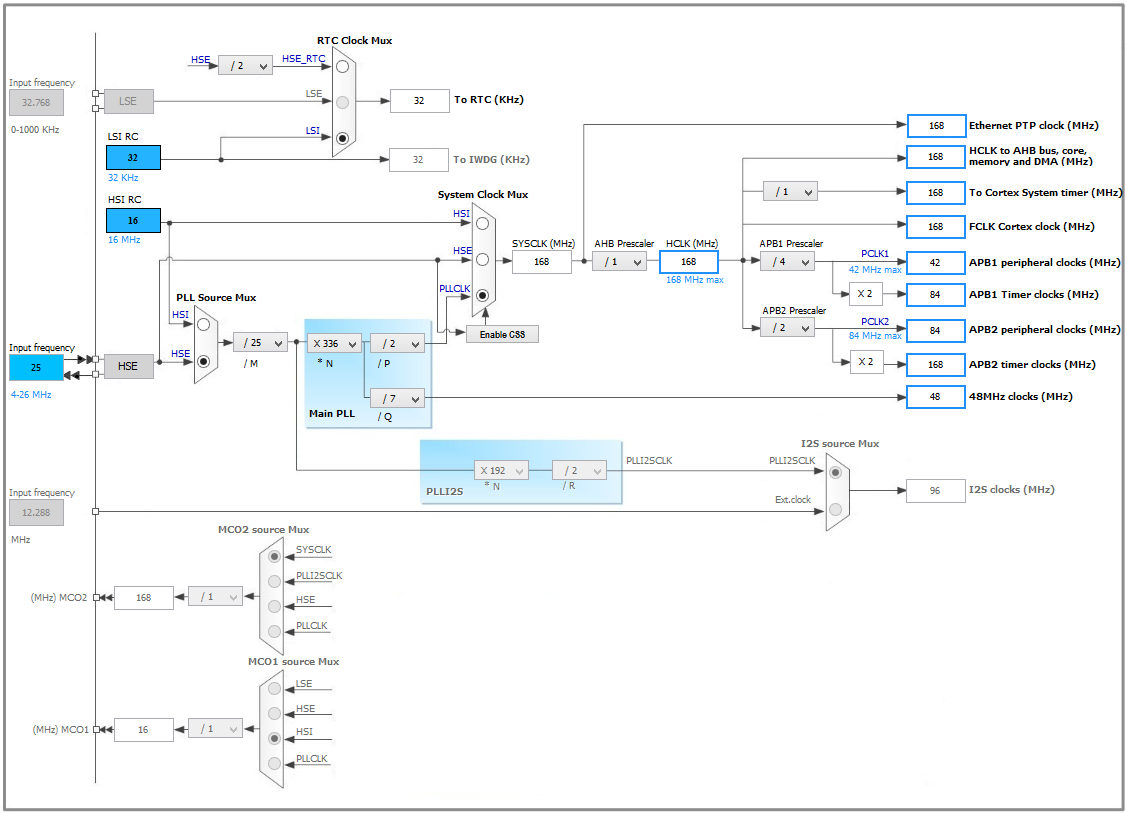
\includegraphics[height=0.43\textheight]{./KonfiguracjaZegara.PNG}
\caption{Konfiguracja mikrokontrolera (zegar) \label{fig:uCclock}}
\end{figure}

\newpage
\section{Konfiguracja peryferiów}
Konfiguracja peryferiów (pokazanych na rysunku \ref{fig:Pery}) została dostosowana do wymagań układów zewnętrznych.
\begin{figure}[!htb]
\centering
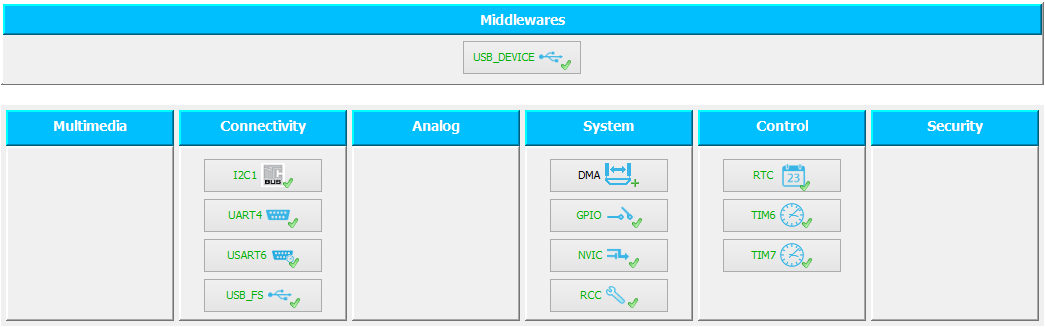
\includegraphics[width=\textwidth]{./KonfiguracjaPery.PNG}
\caption{Konfiguracja peryferiów\label{fig:Pery}}
\end{figure}\\
%\includepdf[pages=5-8]{../AlarmZL41Project/AlarmZL41Project.pdf}
\newpage
\subsection{I2C}
Konfiguracja I2C akcelerometru została przedstawiona w wyciągu z raportu (rysunek \ref{fig:I2C}).
\begin{figure}[!htb]
\centering
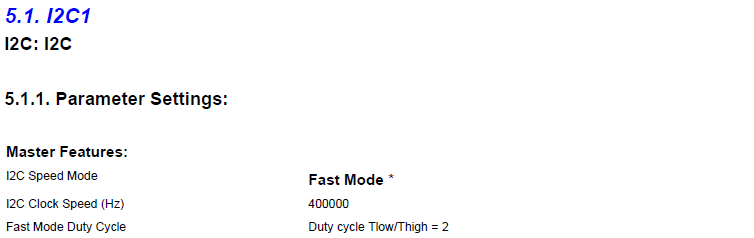
\includegraphics[width=\textwidth]{./KonfiguracjaI2CR.PNG}
\caption{Konfiguracja I2C\label{fig:I2C}}
\end{figure}

\subsection{UART}
Konfiguracja UART dla GSM, GPS oraz komunikacji z komputerem została przedstawiona w wyciągu z raportu (tabela \ref{fig:UART}).
\begin{figure}[!htb]
\centering
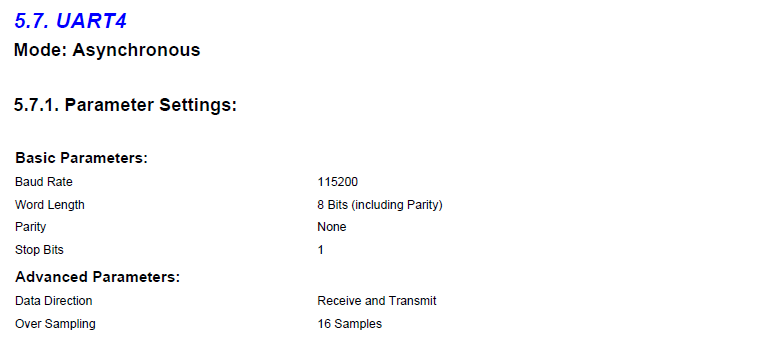
\includegraphics[width=\textwidth]{./KonfiguracjaUARTR.PNG}
\caption{Konfiguracja UART\label{fig:UART}}
\end{figure}
\newpage
\subsection{NVIC}
Konfiguracja przerwań NVIC została przedstawiona w wyciągu z raportu (tabela \ref{tab:NVIC}).
\begin{table}[!htb]
\centering
\caption{Konfiguracja przerwań\label{tab:NVIC}}
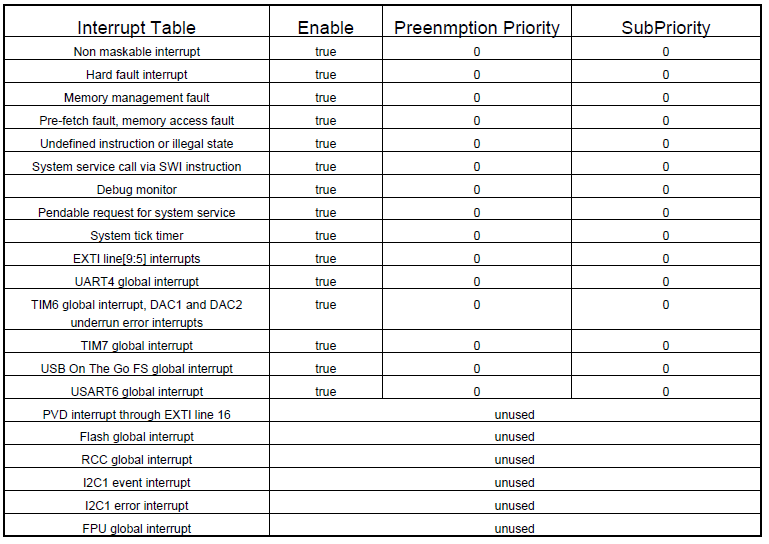
\includegraphics[width=0.75\textwidth]{./KonfiguracjaNVICR.PNG}
\end{table}
\subsection{GPIO}
Konfiguracja GPIO została przedstawiona w wyciągu z raportu (tabela \ref{tab:GPIO}).
\begin{table}[!htb]
\centering
\caption{Konfiguracja GPIO\label{tab:GPIO}}
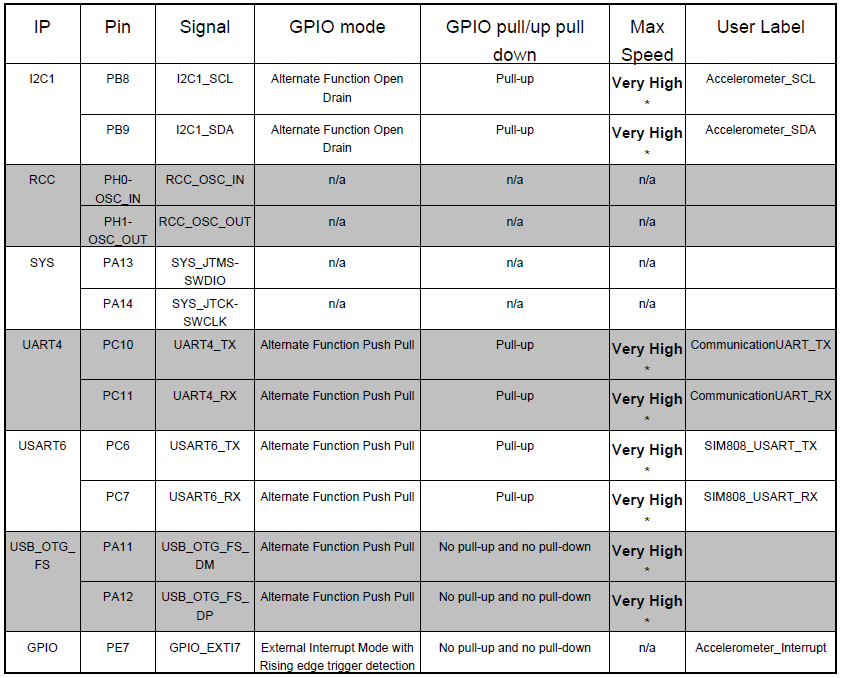
\includegraphics[width=0.75\textwidth]{./KonfiguracjaGPIOR.PNG}
\end{table}
\newpage
\section{Opis układów zewnętrznych}
\subsection{Akcelerometr}
Jako akcelerometr został wykorzystany moduł MPU6050 (rysunek \ref{fig:mpu6050}), komunikujący się po I2C z częstotliwością 400kHz oraz generujący przerwania np. wykrywania ruchu urządzenia (Motion Interrupt). Akcelerometr jest trzyosiowy i jest w stanie mierzyć przyśpieszenia o maksymalnej wartości +/- 16g. 
\begin{figure}[!htb]
\centering
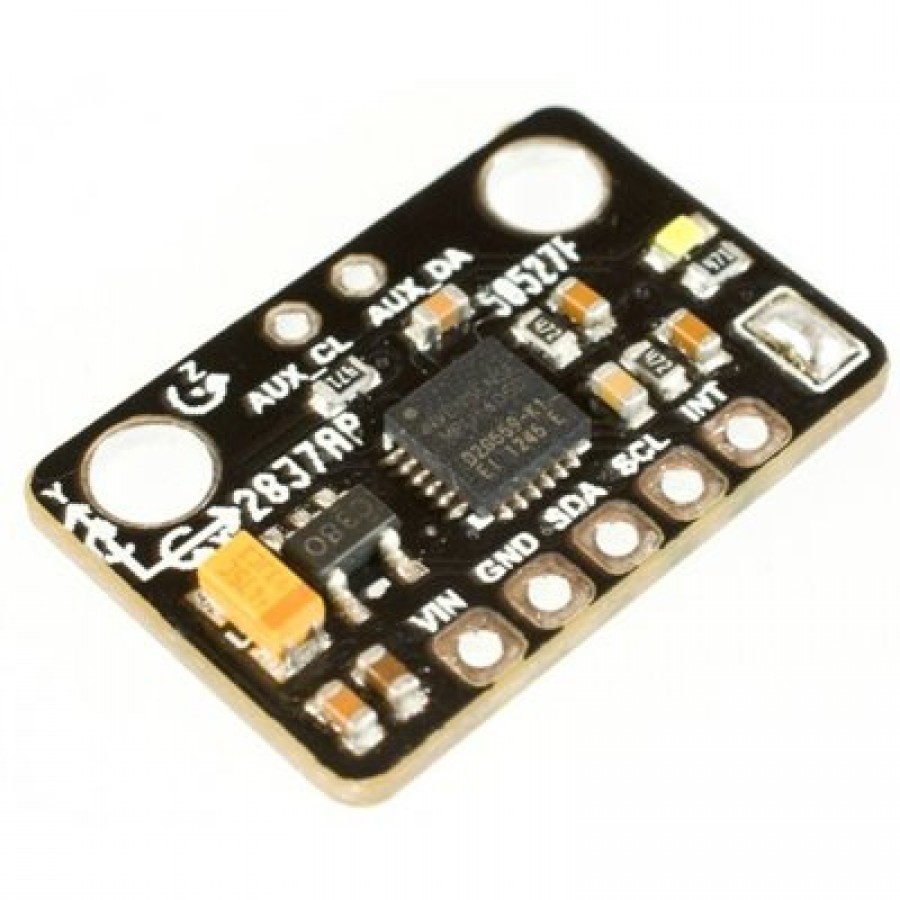
\includegraphics[width=0.4\textwidth]{./mpu6050.PNG}
\caption{Moduł MPU6050 z akcelerometrem\label{fig:mpu6050}}
\end{figure}
Bity konfiguracyjne ustawiane w rejestrach akcelerometru zostały pokazane poniżej.
\lstinputlisting[language=C,firstline=14, lastline=45]{../AlarmZL41Project/Src/Accelerometer.c}
\newpage
\subsection{GSM i GPS}
W projekcie wykorzystano moduł Waveshare sim808 (rysunek \ref{fig:sim808}), z którym można komunikować się za pomocą interfejsu UART oraz przez USB, co zapewnia wbudowany konwerter USB $\rightarrow$ UART. Moduł może być zasilany z zewnętrznego zasilacza, posiada wbudowaną antenę GSM, slot na kartę SIM, oraz możliwość podłączenia anteny GPS. Komunikacja z GSM, a także GPS odbywa się za pomocą komend ''AT''. Weryfikacja poprawności działania po wysłanych komendach odbywa się za pomocą wiadomości zwracanych przez urządzenie (''OK'' oraz ''ERROR'').\\
\begin{figure}[!htb]
\centering
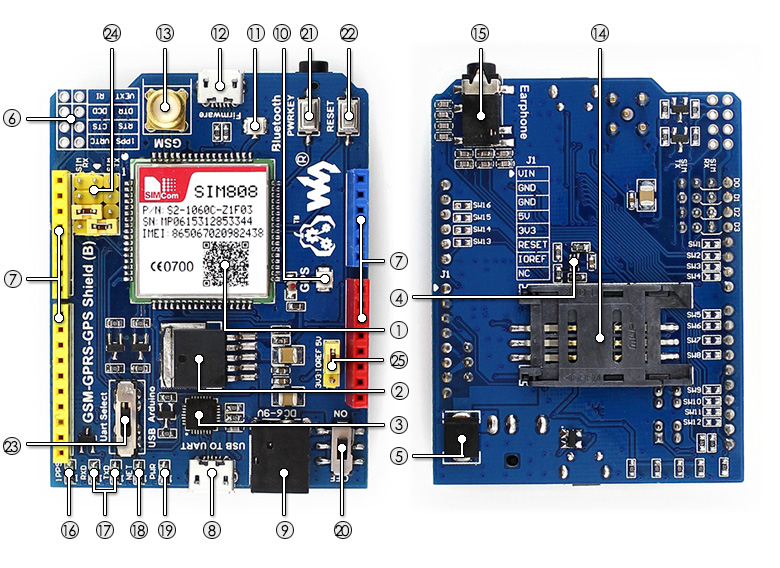
\includegraphics[width=0.9\textwidth]{./Sim808.PNG}
\caption{Moduł Waveshare Sim808\label{fig:sim808}}
\end{figure}\\
Komendy komunikacji z GSM:
\begin{itemize}
\item ''AT'' -- Sprawdzenie poprawności działania urządzenia.
\item \textbf{AT+CLCK=''SC'',1,''pin''} -- Odblokowanie karty SIM.
\item \textbf{AT+CPIN=''pin''} -- odblokowanie karty SIM.
\item \textbf{AT+CMGF=1} -- Podstawowa konfiguracja SMS.
\item \textbf{AT+CMGS=''phone number''} -- Ustawienie numeru telefonu, na który wysłać wiadomość oraz wysłanie wiadomości.
\item \textbf{0x1A} -- Terminator wiadomości. Znak kończący wiadomość SMS.
\end{itemize}

Komendy komunikacji z GPS:
\begin{itemize}
\item \textbf{AT+GSV} -- Sprawdzenie poprawności działania urządzenia.
\item \textbf{AT+CGNSPWR=1}	-- Uruchomienie urządzenia GPS.
\item \textbf{AT+CGNSTST=1} -- Reset GPS. Po tej komendzie GPS zwraca dane co sekundę.
\item \textbf{AT+CGNSINF} -- Pobranie informacji o aktualnej pozycji z GPS.
\item \textbf{AT+CGPSSTATUS} -- Status GPS.
\end{itemize}

\section{Opis działania programu}
\begin{enumerate}
\item Inicjalizacja Akcelerometru (wpisanie do rejestrów urządzenia ustawień ogólnych, poboru mocy oraz przerwań wykrywających ruch).
\item Inicjalizacja GSM (sprawdzenie poprawności działania urządzenia, odblokowanie karty SIM).
\item Inicjalizacja GPS (sprawdzenie poprawności działania urządzenia, wyłączenie urządzenia).
\item Oczekiwanie na przerwania:
\begin{itemize}
\item Odebranie komendy ''log'' lub ''LOG'' przez virtualny port COM USB. 
\begin{enumerate}
\item Wysłanie wszystkich pozycji zapisanych w emulowanej pamięci EEPROM przez USB.
\end {enumerate}
\item Przerwanie od akcelerometru (wykrycie ruchu urządzenia)
\begin{enumerate}
\item Uruchomienie GPS
\item Cykliczne czytanie pozycji urządzenia z GPS i zapisywanie w emulowanej pamięci EEPROM.
\item Uruchomienie timera TIM7, który co określony czas wysyła dzięki GSM, SMS z aktualną pozycją urządzenia.
\end{enumerate}
\end{itemize}
\end{enumerate}

\section{Zadania niezrealizowane}
\begin{itemize}
\item Emulacja pamięci EEPROM w pamięci flash mikrokontrolera.
\item Oprogramowanie i korzystanie z RTC.
\item Stworzenie struktury w pamięci EEPROM przechowującej historie lokalizacji oraz czas z RTC.
\item Pobieranie danych o lokalizacji z modułu GPS.
\item Działający program modułu antykradzieżowego.
\end{itemize}

\section{Bibliografia}
\begin{itemize}
\item \url {https://edu.domski.pl/kursy/sterowniki-robotow/sr-projekt/}
\item G510-GSM-GPRS-command.pdf -- Spis i wyjaśnienie komend ''AT''
\item G510-GSM-GPRS-manual.pdf -- Dokumentacja modułu GSM, GPS
\item quectel-l70.pdf -- Dokumentacja urządzenia GPS Quectel L70
\item quectel-m12.pdf -- Dokumentacja urządzenia GSM Quectel M12
\item STM32F4ReferenceManual -- Dokumentacja miktrokontrolera STM32F417VGT6
\item STM32F7ReferenceManual -- Dokumentacja miktrokontrolera STM32F746VGT6
\item FXOS8700CQManual -- Dokumentacja akcelerometru FXOS8700CQ
\item MPU6050Manual -- Dokumentacja modułu akcelerometru MPU6050
\item MPU6050RegisterMap -- Spis rejestrów modułu akcelerometru MPU6050
\item \url {https://botland.com.pl/arduino-shield-komunikacja/5623-waveshare\\-gsmgprsgps-sim808-shield-nakladka-na-arduino.html} -- Opis i materiały do modułu Waveshare Sim808
\item \url {http://www.waveshare.com/wiki/GSM/GPRS/GPS_Shield_%28B%29} -- Przewodnik użytkownika modułu Waveshare Sim808
\end{itemize}
\newpage
\addcontentsline{toc}{section}{Bibilografia}
\bibliography{bibliografia}
\bibliographystyle{plain}


\end{document}







































